\documentclass[12pt, a4paper]{article}

\usepackage[utf8]{inputenc}
\usepackage{amsmath}
\usepackage{amssymb}
\usepackage{physics}
\usepackage{pgfplots}
\usepackage{mathtools}
\usepackage[hmarginratio=1:1, margin=0.5in, includeheadfoot]{geometry}
\usepackage{float}
\usepackage{wrapfig}
\usepackage{subfig}
\usepackage{setspace}
\usepackage{graphicx}
\usetikzlibrary{decorations.pathreplacing,calligraphy}
\graphicspath{ {./res/} }

\doublespacing % Set line spacing to 1.5

% \usepackage{xcolor}
% \pagecolor[rgb]{0,0,0}
% \color[rgb]{0.5,0.5,0.5}

\title{\vspace{-3cm}Modelling the oscillation of walking humans}
\author{Martin Velikov}
\date{August 2022}

\begin{document}

% title & contents
\maketitle
\tableofcontents

% content
\section{Introduction}
Walking is one of the things that we do most as humans. It is the most
fundamental way of transportation, serving us faithfully for roughly 6 million
years. As one of the few bipedal mammals on the Earth, our motion during walking
is complex and rather effective for the energy we expend doing it. We have tried
to analyze the way we walk, in order to create better tools that, well, enable
us to walk better, like shoes or corrective soles. One fundamental side product
of our peculiar way of motion is that the entire upper body undergoes vertical
oscillation, or put simply, we move and sway up and down whenever we walk.

\subsection{Aim}
The aim of this investigation is, using mathematical functions, to model this
vertical oscillation of the human body while walking.

\subsection{Applications}
There are numerous applications of modern technology where being able to model
the oscillation from walking is invaluable. For example, optical image
stabilization present in nearly all modern video cameras aims to minimize the
'screen shake' by compensating with movement in the lens of the camera. A model
of oscillation while walking could aid this endeavor by allowing more
predictable corrections to be made by software, which would benefit us in
several areas such as film entertainment and physiological analysis.
Additionally, motion discomfort has been a key barrier into the widespread
adoption of virtual reality into our daily lives. Some people do not feel
comfortable in an environment disconnected from their physical presence, and
being able to model a person's sway while walking could aid the endeavor to
smooth, or even recreate it in a virtual world, therefore alleviating this
discomfort and opening the possibilities for a more broad adoption of VR
technology.

\subsection{Personal motivation}
Personally, I am interested in the ways technology can help us in our daily
lives. Being able to reliably apply a model to aid the aforementioned use cases
would be a tremendous achievement that would help integrate technology into
modern lives. 
I also have an interest in physiology \& fitness,
and so being able to apply mathematics to the area is an intriguing \& exciting
opportunity.

\section{Data collection}
\subsection{Background}
In order to model the vertical oscillation of human walking, it must first be
measured accurately. I considered several possibilities for how I can achieve
this, including making a kinematic model of a human leg, or simply filming a
person walking and then tracing over the footage to obtain the path of the leg.
However, both methods posed significant issues with them:
\begin{itemize}
    \item The kinematic model may not be perfectly applicable to the shape,
          proportion \& movement range of a real human leg. It would be very
          complex to make it even approximate the properties of a real human
          leg, which would not be worthwhile since I would only be trying to
          extract data from it once or twice.
    \item Tracing over a film of someone walking poses some accuracy \&
          precision errors. For example, determining the location of the part of
          the leg that needs to be tracked would rely on a visual estimate,
          which is subject to the many issues of a video camera, such as
          parallax error (as an orthographic camera cannot physically exist),
          motion blur, resolution \& lens distortion.
\end{itemize}

\subsection{Solution}
In order to address the issues with the initially proposed data collection
methods, I opted for a more robust \& accurate to real life measurement technique
of actually motion tracking in 3D while walking. For the purposes of this
investigation, I did not require full limb-for-limb tracking - only my head, and
the bases of my feet. \\

For the task, I used an Oculus Rift virtual reality headset and motion
controller pair in an improvised setup. Although the controllers are meant to be
used for hand tracking, I fixed them securely to my ankles, as close as possible
to my heel, and found that they still tracked the motion of walking accurately.
\\

For the software, after some research on what popular dance groups such and
other "fully virtual dancers" use, I found that they all used the same set of
software, albeit with a more elaborate setup than my improvised one.

\begin{figure}[H]
    \centering
    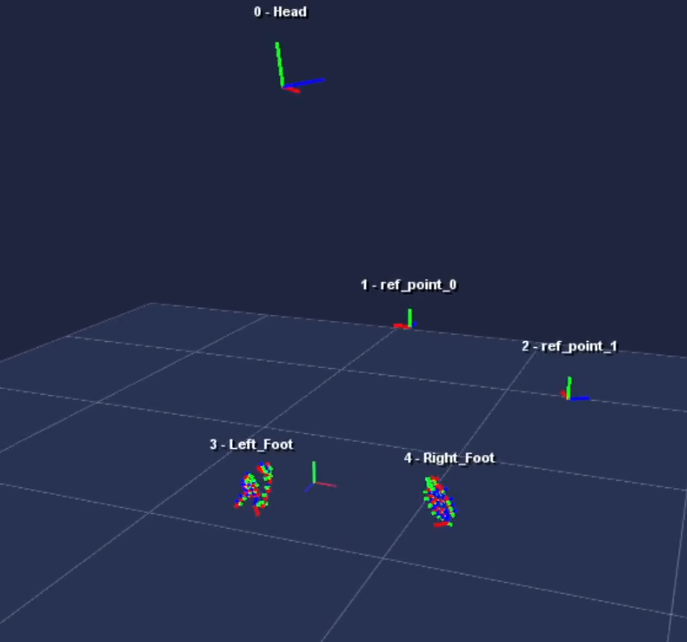
\includegraphics[width=8cm]{mocap_software}
    \caption{Motion tracking setup with person in the middle of a step}
    \label{mocap}
\end{figure}

Figure \ref{mocap} shows the computer side of the tracking setup. I used two IR
tracking sensors (\texttt{ref\_point\_0} and \texttt{ref\_point\_1}) pointed at
the area I was to walk through, and set up the software so that it tracked my
head and feet, to which the tracking points were attached to.

After some testing with moving the tracking point along a ruler, I found that
the position data returned was accurate to two millimeters, which is far beyond
anything that would have been achieved with the two initially proposed data
collection methods.

\subsection{Results}
\label{results}

\begin{figure}[H]
    \centering
    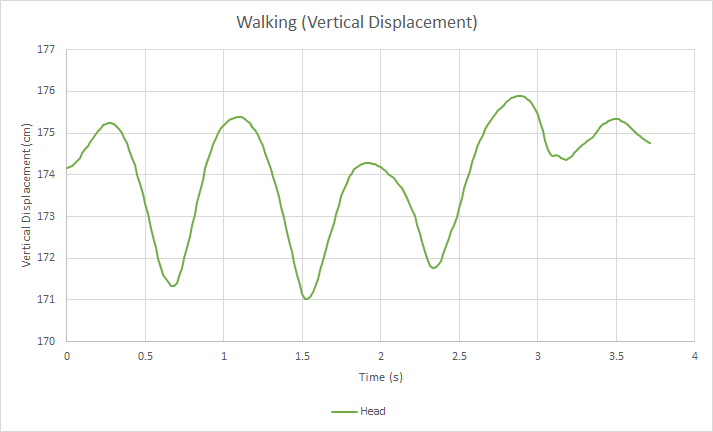
\includegraphics[width=12cm]{head_vert.png}
    \caption{Vertical motion of head}
    \label{head_y}
\end{figure}

Figure \ref{head_y} depicts the vertical displacement of my head from the floor.
It can be observed that it resembles some sort of wave with crests \& troughs,
which makes sense - a person walking would go up and down periodically with
every step. From the graph, it is evident that the 4 steps were taken, indicated
by the 4 crests. It is also noteworthy that the troughs are far sharper than the
crests, which may be a product of the foot of the walker hitting the floor (the
trough), and the leg moving through the air (the crest). Anyhow, this
interesting pattern warrants investigation, as the head is the best indicator of
the general vertical motion of the body in this case.

\begin{figure}[H]
    \centering
    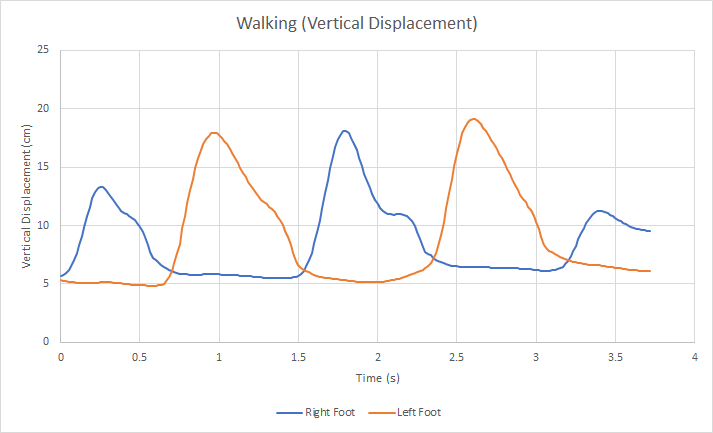
\includegraphics[width=12cm]{feet_vert.png}
    \caption{Vertical motion of feet over time}
    \label{feet_y}
\end{figure}

Figure \ref{feet_y} depicts the motion of my feet vertically. It is evident from
this that each foot has two crests, for a total of four steps, which matches up
nicely with the observations made from Figure \ref{head_y}. The shape of these
crests and troughs is peculiar, but anyhow seem to follow an explicable pattern.
It seems like the graphs of the right and left foot are completely out of phase,
which makes sense given that only one foot can be on the ground at a time,
during which the other one must be in the process of taking a step. \\

The shape of the troughs makes sense as well, as they are almost perfectly flat.
The small amount of curvature that precedes the large peak is most likely caused
by the heel being lifted in the air as the foot is getting ready for another
step. This is further supported by the fact that at the beginning, the left
foot's first trough is far sharper than the succeeding ones, because one leg of
the person walking would be starting the step from a standstill.

It is also noteworthy to talk about the small secondary bump following the
crest, visible in all crests, but most prominent in the second step of the right
foot. This could be explained as the foot of the person walking maintaining an
approximate level height, then suddenly returning to the ground on the
"falling edge" of a step. In reality, the prominence of this secondary bump
could be specific to the walking style of the person, however, it is significant
enough to the point where it cannot be disregarded as simple error.

\begin{figure}[H]
    \centering
    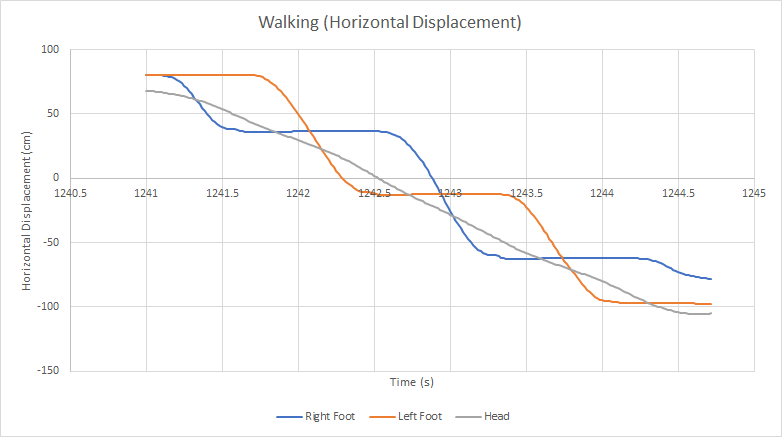
\includegraphics[width=13cm]{motion_horiz.png}
    \caption{Horizontal motion of ankles and head}
    \label{horiz}
\end{figure}

Figure \ref{horiz} shows the horizontal motion of the three tracked points
throughout the walk. Its data is not necessarily relevant to modelling the
vertical oscillation, however it is able to provide some key insights into the
motion of the person during the walk. It is evident that generally, for all
three graphs, the motion happens in one direction, which is forward, or, on the
graph, towards $-\infty$. The graphs of horizontal motion of the feet alternate
in successive "dips", which resemble one step, where one foot is stationary
while the other is free to move forward. The graph of the motion of the head is
very close to being linear, and it appears to pass through the graphs of both
feet. In the regions where the graph of a foot is above the graph of the head,
it would be lagging behind in real life, while being below would mean it is
ahead. Generally, it can be observed that the regions where it is found above
the graph of the head (lagging behind) are greater than the regions where it is
behind, which coincides with the data for the vertical motion of the feet, where
the falling edge of each crest is generally longer than its rising edge.

\section{Modelling options}
In terms of modelling the curves, a polynomial may prove to provide the most
precise model of the dataset, especially for the more peculiar graphs like those
of the motion of the feet. There are three main advantage of using polynomials
to model these motions. First, polynomials are inexpensive to compute and work
with, since they only use multiplication and addition, something both humans and
computers are quite adept at. This makes representing something as a polynomial
very worthwhile. Based off of this, the second advantage - fitting polynomials
to best approximate data is a well-explored topic, with several well-established
working methods which can be used to provide shockingly accurate results. The
last of these advantages is specific to the shape of our graph - it has smooth
curves, which polynomials are excellent at representing. \\

There are several relatively easy methods to fit polynomials to a function,
supposing that you can find its derivative. One possible method is constructing
a Taylor polynomial, which would be accurate around the point which is
constructed. Unfortunately, for our case, we are trying to fit through a dataset
of points, for which finding the derivative (or more importantly, higher-order
derivatives) might prove challenging without, paradoxically, knowing how to
define the original function. \\

Ultimately, the method that is most applicable to this type of task is some type
of regression. Since we are trying to fit a polynomial to the data, polynomial
regression with some cost function will work nicely. For the cost function, the
"least squares" has been chosen for its simplicity, effectivity and widespread
use.

% \pagebreak
\section{Least squares polynomial fitting}
\subsection{Theory}
Suppose that there is a polynomial $P$ of degree $k$ so that
\begin{align*}
    P(x)= a_0 + a_1 x + \cdots + a_{k-1} x^{k-1} + a_k x^k
\end{align*}


\begin{wrapfigure}[12]{r}{7cm}
    \centering
    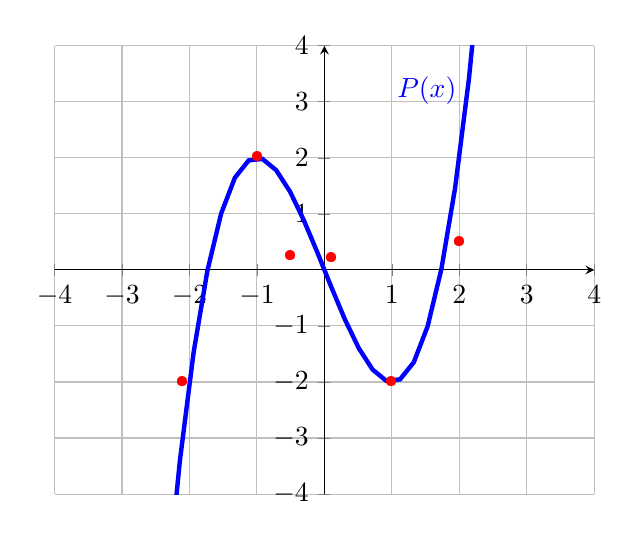
\begin{tikzpicture}
        \begin{axis}[
                axis y line=center,
                axis x line=middle,
                xmin=-4,
                xmax=4,
                ymin=-4,
                ymax=4,
                % height=12.0cm,
                % width=12.0cm,
                grid,
                xtick={-4,...,4},
                ytick={-4,...,4},
            ]
            \addplot [domain=-5:5, samples=50, mark=none, ultra thick, blue] {x^3-3*x};
            \node [left, blue] at (axis cs: 2.1, 3.2) {$P(x)$};
            \node [red] at (axis cs: 1, -2) {\textbullet};
            \node [red] at (axis cs: 2, 0.5) {\textbullet};
            \node [red] at (axis cs: -0.5, 0.25) {\textbullet};
            \node [red] at (axis cs: -2.1, -2) {\textbullet};
            \node [red] at (axis cs: 0.1, 0.2) {\textbullet};
            \node [red] at (axis cs: -1, 2) {\textbullet};
        \end{axis}
    \end{tikzpicture}
    \caption{
        Example cubic ($k=3$) $P(x)$ fitting 5 points.
    }
    \label{fig1}
\end{wrapfigure}

The coefficients $a_0$ through $a_k$ are the unknowns that must be solved for,
defining the shape of the polynomial. Assuming one wants to fit this polynomial
to a set of points, it would be useful to know how accurately it can model the
dataset, given a guess of its coefficients $a_0 \cdots a_k$.

Figure \ref{fig1} depicts one such cubic polynomial. It is evident from the
graph that $P(x)$ does not exactly pass through every point - rather, there is a
slight difference for every point it passes by. Let one of these points be
represented as $(x, y)$. The vertical difference $r$ between this point and the
graph of $P$ could be simply represented by

\begin{align*}
    r=|y-P(x)|
\end{align*}

The absolute value of the difference is used since $r$ should be indicative of
the deviation from the graph, therefore the direction of difference is
irrelevant. Furthermore, instead  of taking the modulus of the right side, it
can simply be squared in order to accentuate any error, but more importantly be
derivable, as the absolute value produces discontinuous derivatives. (Weisstein,
2022) This leaves the final equation of the difference $r$ between a point $(x,
y)$ as

\begin{align*}
    r=(y-P(x))^2
\end{align*}

The total measure of deviation $R^2$ from the graph $P(x)$, called the
"residual", can be obtained by summing up the aforementioned vertical
differences for $n$ points with coordinates $(x, y)$: (Weisstein, 2022)

\begin{align*}
    R^2 & = \sum^n_{i=1}[y_i-P(x_i)]^2 \\
    % &= \sum^n_{i=1}[
    %     y_i - (a_0 + a_1 x_i + \cdots + a_{k-1} x_i^{k-1} + a_k x_i^k)]^2
\end{align*}

The partial derivative of the residual with respect to each coefficient can be
found, and set to zero in order to ensure that coefficient contributes a minimum
of the error in terms of the entire equation - this effectively minimizes $R^2$,
which is the goal of this method. This results in the following system of
equations with partial derivatives that must be brought to zero: (Weisstein, 2022)

\begin{align*}
    \pdv{(R^2)}{a_0}     & = -2 \sum^n_{i=1}[y_i-P(x_i)] x^0     & = 0 \\
    \pdv{(R^2)}{a_1}     & = -2 \sum^n_{i=1}[y_i-P(x_i)] x^1     & = 0 \\
                         & \vdotswithin{=}                             \\
    \pdv{(R^2)}{a_{k-1}} & = -2 \sum^n_{i=1}[y_i-P(x_i)] x^{k-1} & = 0 \\
    \pdv{(R^2)}{a_k}     & = -2 \sum^n_{i=1}[y_i-P(x_i)] x^k     & = 0
\end{align*}

From this point, the method requires solving the above system for the most
closely fitting coefficients, i.e. minimizing $R^2$. There are several methods
through which this system of equations can be simplified and solved, the proof
of which, however, is beyond the scope of this investigation. After
simplification, the matrix system can be represented as (Weisstein, 2022)

\begin{align*}
    \begin{bmatrix}
        1      & x_1     & x_1^2     & \cdots & x_1^{k-1}     & x_1^k     \\
        1      & x_2     & x_2^2     & \cdots & x_2^{k-1}     & x_2^k     \\
        \vdots & \vdots  & \vdots    & \ddots & \vdots        & \vdots    \\
        1      & x_{n-1} & x_{n-1}^2 & \cdots & x_{n-1}^{k-1} & x_{n-1}^k \\
        1      & x_n     & x_n^2     & \cdots & x_n^{k-1}     & x_n^k
    \end{bmatrix}
    \begin{bmatrix}
        a_1 \\ a_2 \\ \vdots \\ a_{k-1} \\ a_k
    \end{bmatrix}
    =
    \begin{bmatrix}
        y_1 \\ y_2 \\ \vdots \\ y_{n-1} \\ y_n
    \end{bmatrix}
\end{align*}

An interesting point about this method is that if the number of points $n$ that
the polynomial must be fit to exceed the degree $k$, the polynomial can never
pass through all of them exactly, which makes sense given that the polynomial
may only have a maximum of $k-1$ turning points. This means that the above
system of matrices is "over-determined", that is, it can never give a perfect
solution in terms of coefficients, only the closest approximation. \\

As for solving the system, multiplying by the transpose $X^T$ of the matrix with
x-terms $X$ would yield a square linear system which can then be solved
numerically for the coefficients in the vector $\vec{a}$.

\begin{align*}
    X^TX\vec{a}=X^T\vec{y}
\end{align*}

As mentioned above, and in the case that applies to solving this problem, a
well-formed solution to this system does not exist most of the time. However, if
the degree $k$ is greater than $n$, the system can be solved for a single vector
of solutions by simply inverting $X^TX$:

\begin{align*}
    \vec{a}=(X^TX)^{-1}X^T\vec{y}
\end{align*}

\subsection{Application \& Exploration}
Now that the underlying method that powers this type of polynomial regression is
known, it is possible to apply it to the dataset. While a polynomial might
accurately model one crest or trough of a step, in reality it would not be
practical to model the entire collected data-set with just one. There are
several methods to account for this issue which will be explored below. \\

As for actually fitting the polynomials using the above method, I wrote a
computer program in the Python programming language which solved the system
using the NumPy mathematics library and MatPlotLib for visualization. I further
used MATLAB to draw some figures and draw insights.

\subsubsection{Even "naive" subdivision}
\label{section_naive_seg}
A naive solution to the problem is to segment the entire domain into even
chunks, then fit a polynomial to the portion of the graph (drawn as a punctured
line) in those subregions (divided vertically with dotted lines):

\begin{figure}[H]
    \centering
    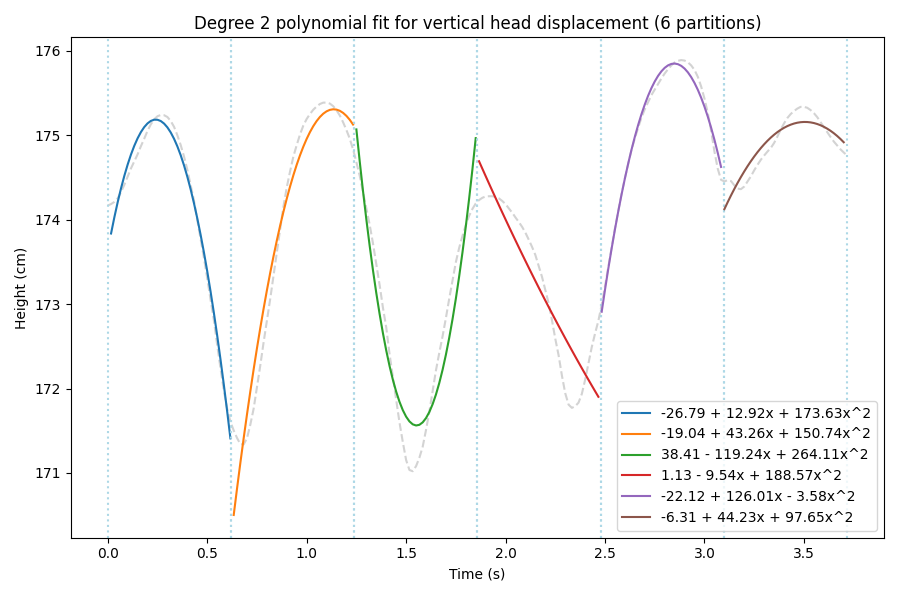
\includegraphics[width=12cm]{p_naive_head_2.png}
    \caption{Naive quadratic fitting for vertical head oscillation data}
    \label{naive_head}
\end{figure}

\begin{figure}[H]
    \centering
    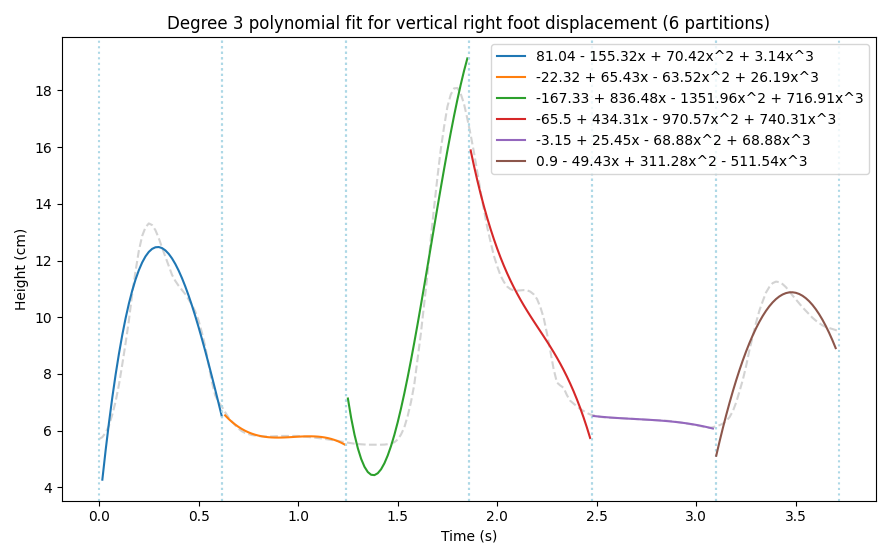
\includegraphics[width=12cm]{p_naive_right_3.png}
    \caption{Naive cubic fitting for vertical right foot oscillation data}
    \label{naive_right}
\end{figure}

There are several main observations that can be made from these naive fitting
attempts: first, from Figure \ref{naive_head}, it is evident that all crests and
troughs are smooth and symmetrical enough so that a quadratic can accurately
model them. This should be kept in mind as it will become important when trying
to refine the fitting method. While the first crest in Figure \ref{naive_head}
appears to be well-fitted, the same cannot be said for the succeeding crests or
troughs.

A possible explanation for this is that the selection of subregions does not
respect any of the graph features that a quadratic might benefit from, like the
aforementioned smooth curvature at the crests and troughs. For example, the
third crest's equation (red) is a quadratic that acts very similarly to a linear
in the region it is meant to approximate, since there are not enough turning
points for it to assume the necessary shape. The result of this, as we can see,
is not a very good fit.

In the more complex graph of Figure \ref{naive_right}, this is further
reciprocated. Even though a higher degree of polynomial is used, some regions of
the graph are fitted far better than others, like the first crest compared to
the second, which, due to the naive segmentation, is forcefully cut in two.  \\

While this method is a good start, it has a plethora of shortcomings which can
be addressed quite easily. In general, the fit of the graph is quite poor.

\subsubsection{Crest \& trough subdivision}
\label{crest_trough_subdivision}
In order to address the issues found in \ref{section_naive_seg}, and take
advantage of the patterns identified, we are going to have to examine our
dataset more closely. Polynomial functions are able to fit a dataset
much more closely if the area over which they are fitted is of a similar shape
to them. For example, curved crests and troughs are present in the dataset here,
and they can almost perfectly be fit by a quadratic.

\begin{figure}[H]
    \centering
    \subfloat[\centering Example of a quadratic that fits the crest well]{
        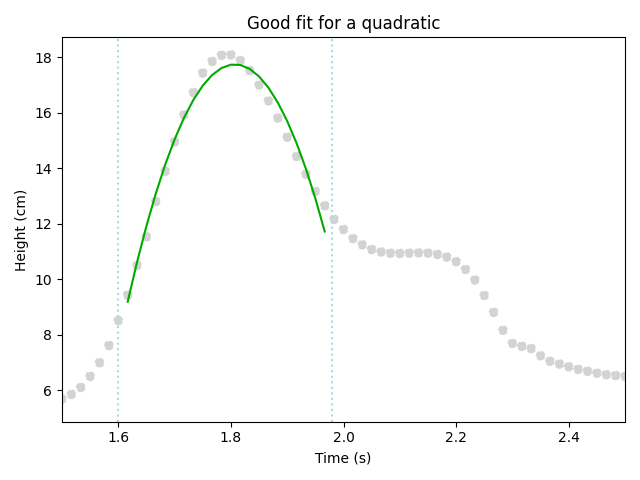
\includegraphics[width=0.5\textwidth]{good_fit.png}
        \label{good_quadratic}
    }
    \subfloat[\centering Example of a quadratic with a poor fit]{
        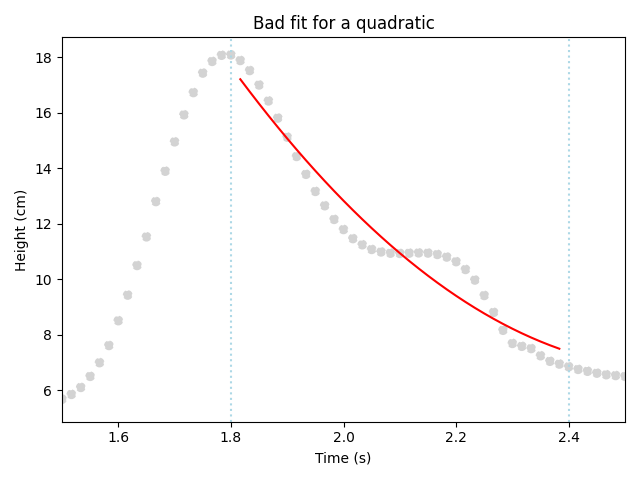
\includegraphics[width=0.5\textwidth]{bad_fit.png}
        \label{bad_quadratic}
    }
    \caption{ Examples of how the region over which a polynomial is fit can
        drastically affect the accuracy of the fit }
    \label{bad_good_quadratics}
\end{figure}

In Figure \ref{good_quadratic}, the crest can be perfectly fit by a concave down
quadratic, as the region in which the regression was performed was limited to
just around the crest. In contrast, Figure \ref{bad_quadratic} shows a misplaced
quadratic that is trying to fit an area not suited for its shape, resulting in
heavy deviations from the data.

Knowing this, it is possible to improve the segmentation method to look for
areas that might be a good fit for specific polynomial functions. For a
quadratic, looking for the crests and troughs to harness the aforementioned
benefits from their shape is a good staring point.

Crests and troughs can be considered the local minima and maxima of the data at
their peaks. It is a property of functions that these minimum and maximum points
are also turning points, meaning the derivative of the function changes sign
around them. Applying this to the current data, it is sufficient to find a point
around which both neighboring points are either both above or both below in the
y-axis, as this effectively compares if the slopes of the two neighboring
points relative to the central point have inverted.

\begin{figure}[H]
    \centering
    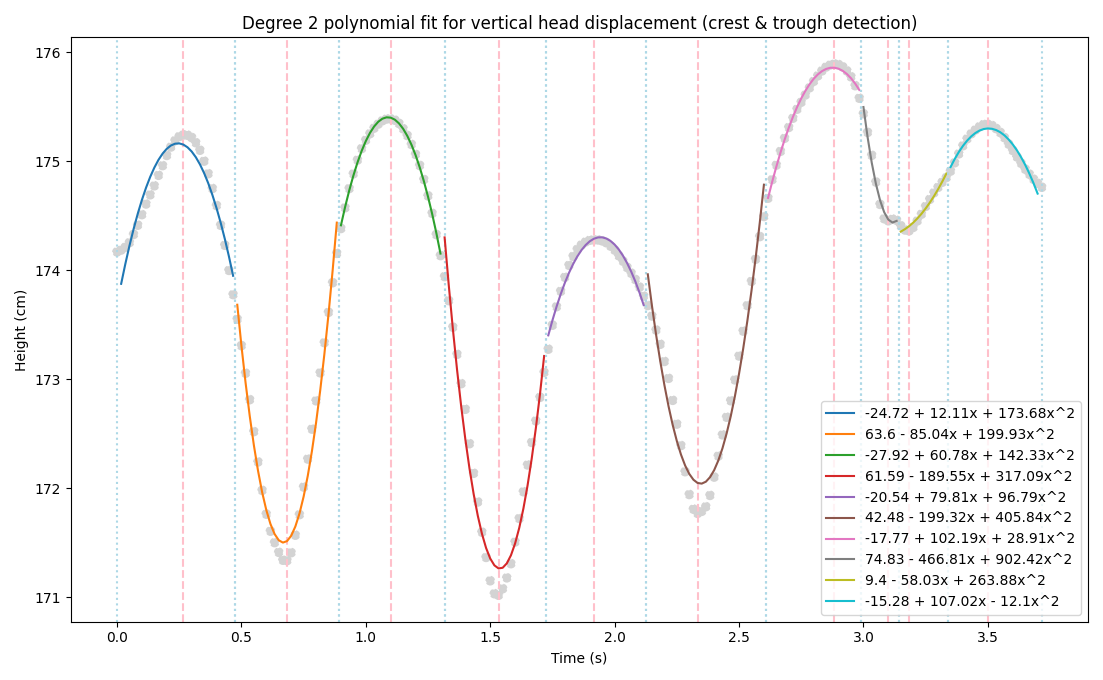
\includegraphics[width=14cm]{p_peaks_head_2.png}
    \caption{ Quadratic fitting for vertical head oscillation data with crest \&
        trough detection}
    \label{peaks_head}
\end{figure}

Figure \ref{peaks_head} demonstrates this detection method in action - the red
dashed vertical lines show the point at which a crest or trough was detected,
and the blue dotted lines show the start \& end of each fitting region. These
region borders are placed between each crest or trough, by averaging their
x-coordinates. Compared to the naive fit seen in Figure \ref{naive_head}, this
is certainly a much better outcome as we can see the quadratics' curves being
used more effectively around the peaks.

\begin{figure}[H]
    \centering
    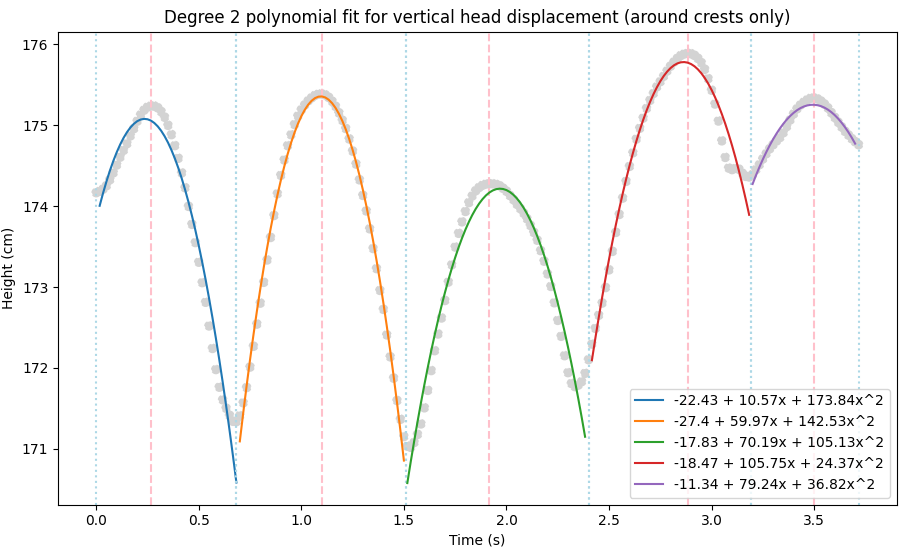
\includegraphics[width=14cm]{p_peaks_crestsonly_head_2.png}
    \caption{ Quadratic fitting for vertical head oscillation data with crest
        detection only }
    \label{crestsonly_head}
\end{figure}

The sharpness of the troughs seen in the head movement data poses an interesting
question - how would the accuracy of the model vary if only the crests were used
as the bases around which the quadratic are to be fit? Figure
\ref{crestsonly_head} illustrates one such example, and interestingly, it seems
that even with this, virtually no important information appears to be lost, yet
the number of equations has been reduced to half, all of which are, naturally,
concave down.

\begin{figure}[H]
    \centering
    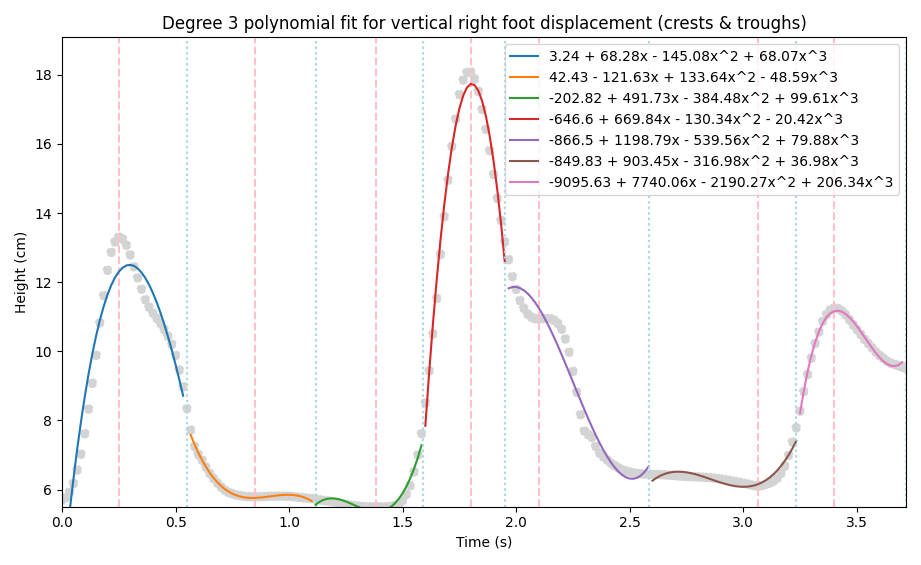
\includegraphics[width=14cm]{p_peaks_right_3.png}
    \caption{ Cubic fitting for vertical right foot oscillation data with crest
        \& trough detection }
    \label{peaks_right}
\end{figure}

Figure \ref{peaks_right} shows the vertical oscillation of a right foot, with
cubics fitted using the new method. It can be seen that with crest \& trough
detection, the results are still much more accurate than the naive approach.
However, it should be noted that the data for the motion of feet is
significantly more complex to model than the data for the head, hence the
comparative inaccuracy of the fit. In the end, even though there is some
evidence of improvement from the previous method for dividing subregions for the
vertical oscillation of the feet, it is still too inaccurate to be used for the
final model.

\subsubsection{Manual subdivision}
Although a fitting solution has been found for the graph of the vertical
oscillation of the head while walking (Figure \ref{crestsonly_head}), in order
to fit a polynomial to the more complex graphs of the feet, a more precise
method is required. \\

As the crests observed in these graphs appear to repeat over a period, it would
potentially be useful to fit a polynomial to one of these by manually specifying
the domain. This would then allow us to extrapolate the fitted polynomial to
other crests, and apply the insight learned from the previous attempts at
fitting. \\

\begin{figure}[H]
    \centering
    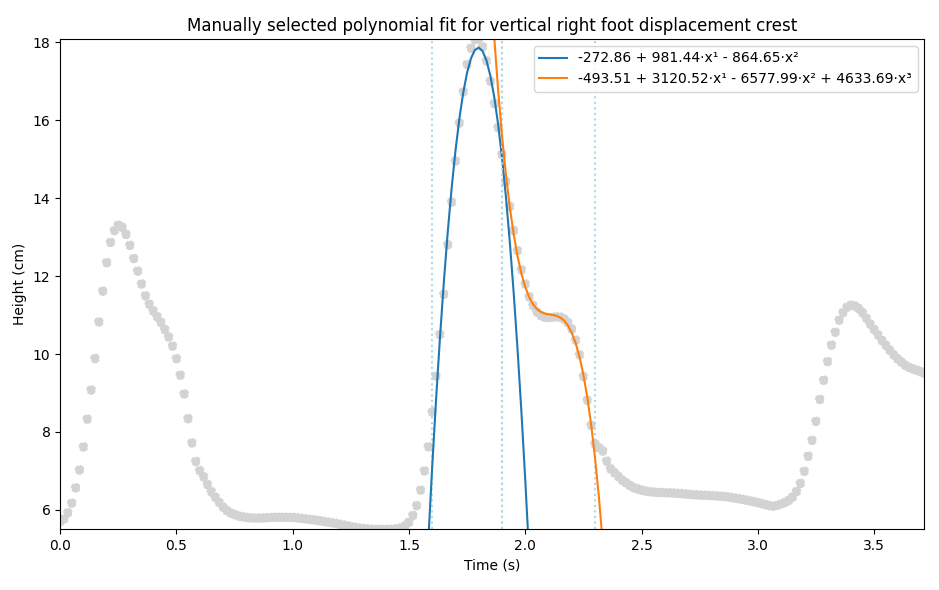
\includegraphics[width=14cm]{p_manual_right.png}
    \caption{ Cubic \& quadratic fitting for vertical right foot oscillation
        data by manually selecting the fitting region }
    \label{manual_right}
\end{figure}

Figure \ref{manual_right} demonstrates a manual fit of a quadratic for $1.6 \le
    x \le 1.9$ and a cubic for $1.9 \le x \le 2.3$. Based on the knowledge of the
efficacy of concave down quadratics at modeling crests explored in Section
\ref{crest_trough_subdivision}, a quadratic has been used in that region, which
appears to fit well. Similarly, a flat area can be observed to the right of the
peak, which happens to almost perfectly be modelled by a cubic, with a
stationary point in the middle of the flat area. From these results, it is safe
to say that this combination of a quadratic and cubic is sufficient to model the
crests of vertical oscillation in feet.

\subsection{Assembling}
In order to assemble the final model for the vertical oscillation while walking,
we can draw on the best fitting methods to model the oscillation of the head and
feet. For the head, the "crest-only concave down quadratic" fit depicted in
Figure \ref{crestsonly_head} seems like the best choice due to how accurately it
represents the original data using very few quadratic equations. \\

\subsubsection{Head vertical oscillation}
The quadratic equations returned by the regression process are in standard form.
In order to make the equations more wieldy to work with, it would be sensible to
convert them into vertex form, as this gives us the coordinate of the crest's
peak, which can prove useful if we're trying to figure out the periodicity of
the dataset. \\

For this conversion, it is a good start to first find the roots $r_1$ and $r_2$
of the quadratic $Q(x)$ using the quadratic formula:


\begin{align*}
    \text{Given $Q(x) = ax^2 + bx + c$,} \\
    \Delta = b^2 - 4ac                   \\
    r_1    = \frac{-b + \sqrt{\Delta}}{2a},
    r_2    = \frac{-b - \sqrt{\Delta}}{2a}
\end{align*}

As the vertex lies perfectly in the middle of the two roots, finding its
x-coordinate $h$ is easy to do by just averaging the roots:
Then, evaluating $Q(h)$ would also give us the y-coordinate $k$ of the vertex.

\begin{align*}
    h & = \frac{r_1 + r_2}{2}  \\
    k & = Q(h) = ah^2 + bh + c
\end{align*}

Using the values for $h$ and $k$, it is now possible to express the original
quadratic in the vertex form $Q(x)=a(x-h)^2+k$. Evaluating this for the first
two equations $Q_1(x)$ and $Q_2(x)$ fit to the crests of the vertical head
oscillation data:

\begin{align*}
    Q_1(x) & = -22.43x^2 + 10.57x + 173.84                                                                                                          \\
    \Delta & = 10.57^2 - 4(-22.43)(173.84) \approx 15708.650                                                                                        \\[5mm]
    r_1    & \approx \frac{-10.57 + \sqrt{\Delta}}{2(-22.43)}                         \qquad  r_2  \approx \frac{-10.57 + \sqrt{\Delta}}{2(-22.43)} \\
    r_1    & \approx -2.558                                                           \qquad\qquad\quad\thinspace  r_2  \approx 3.030               \\[5mm]
    h      & \approx \frac{-2.558 + 3.03}{2} \approx 0.236                                                                                          \\
    k      & = Q(h) \approx -22.43(0.236)^2 + (10.57)(0.236) + 173.84 \approx 175.085                                                               \\[5mm]
    Q_1(x) & \approx -22.43(x - 0.236)^2 + 175.085
\end{align*}

Applying the same process for $Q_2(x)$, \quad $Q_2(x) \approx -27.4(x - 1.094)^2 + 175.344$. \\

As noted by the discussion in \ref{results}, the pattern observed in all
collected data appears to be cyclical. Here, this is further reciprocated as the
values of $a$ for both $Q_1$ and $Q_2$ are very similar, potentially alluding to
the fact that all peaks are roughly the same in shape.

This means that it may be a valid approach to represent it as a series of the
same equations with a constant offset, called the "period". We can use the
already found coordinates of the vertices of $Q_1$ and $Q_2$ to find the value
of the period $p$.

\begin{figure}[H]
    \centering
    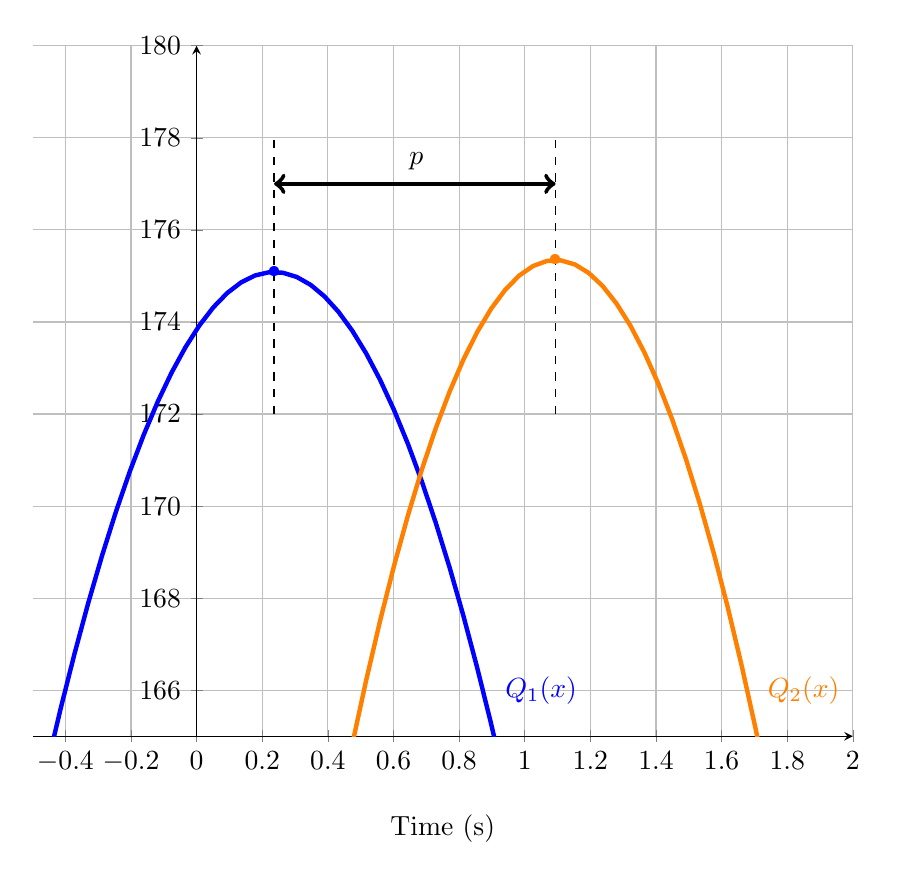
\begin{tikzpicture}
        \begin{axis}[
                axis y line=middle,
                axis x line=bottom,
                xmin=-0.5,
                xmax=2,
                ymin=165,
                ymax=180,
                width=12cm,
                samples=60,
                no markers,
                grid,
                x label style={at={(axis description cs:0.5,-0.1)},anchor=north},
                y label style={at={(axis description cs:-0.1,.5)},rotate=90,anchor=south},
                xlabel={Time (s)}]
            ylabel={Height (cm)},
            ]
            \addplot [domain=-0.5:2, ultra thick, blue] {-22.43*(x - 0.236)^2 + 175.085};
            \node [blue] at (axis cs:1.05,166) {$Q_1(x)$};
            \addplot [domain=-0.5:2, mark=none, ultra thick, orange] {-27.4*(x-1.094)^2+175.344};
            \node [orange] at (axis cs:1.85,166) {$Q_2(x)$};

            \draw [dashed] (axis cs:0.236,172) -- (axis cs:0.236,178);
            \draw [dashed] (axis cs:1.094,172) -- (axis cs:1.094,178);
            \draw [<->,  ultra thick] (axis cs:0.236,177) -- (axis cs:1.094,177);
            \node at (axis cs:0.67,177.5) {$p$};

            \node [blue] at (axis cs:0.236,175.085) {\textbullet};
            \node [orange] at (axis cs:1.094,175.344) {\textbullet};
        \end{axis}
    \end{tikzpicture}
    \caption{ Graphs of $Q_1$ and $Q_2$. $p$ is the horizontal
        distance between their vertices. }
    \label{vertexforms}
\end{figure}

Figure \ref{vertexforms} shows how it is possible to figure out the period of
vertical head oscillation by finding the horizontal distance between the two
vertices. In terms of the original function of the vertical head displacement,
the vertices are the peaks of the graph, where the cycle of the function appears
to repeat.

Calculating $p$ by subtracting $Q_1$'s vertex x-coordinate $h_1$ from
$Q_2$'s vertex x-coordinate $h_2$, it can be found that $p = 1.094 - 0.236 = 0.858$.

As the x-coordinate here represents the time in seconds, the value of $p$ tells
us that a full step of the walking cycle takes around 0.858 seconds, or 858
milliseconds, which seems to be inline with what can approximately be observed
in real life - it takes about a second to take a full step. \\

Using the property that $p$ denotes a period, it is then possible to create a
series of equations $y_0 \dots y_n$ which describe the step accurately at different points in
time $x$.

\begin{align*}
    y_0 & = at^2 + k                                \\
    y_1 & = a(x-p)^2 + k                            \\
    y_2 & = a(x-2p)^2 + k                           \\
        & \phantom{t=\,} \vdots                     \\
    y_n & = a(x-np)^2 + k \qquad n \in \mathbb{Z} \\
\end{align*}

The value of $a$ defines the shape of the steps. It is reasonable to assume that
this value depends on the physical parameters of the person walking. From the
data collected, we can calculate the mean of $a$ values for $Q_1$ and $Q_2$ and
use it as a good enough estimate. $a = \frac{-22.43 -27.4}{2} = -24.915$ \\

Furthermore, by subtracting $p$ along the values of $t$, the graph of any $y_0
\dots y_n$ is horizontally translated right by $p$ with each succeeding
equation. This means that value of $p$ determines the period between each step,
which effectively makes it represent how fast the person walking can take steps.
This is again dependent on the person, but for our dataset we will use the
previously obtained value $p=0.858$. If a generalization is necessary, one can
use $p = h_2 - h_1$. \\

The value for $k$ denotes the maximum height any equation $y_0 \dots y_n$ will
reach, as all of their vertices will have the y-coordinate $k$. As the height of
the head from the floor will be at a maximum whenever the person's leg is fully
extended, the value of $k$ can simply be taken as the person's standing height.
Similarly to how $a$ was computed here, $k$ can be gotten by averaging the
y-coordinates of the vertices of $Q_1$ and $Q_2$: $k = \frac{175.085 +
        175.344}{2} = 175.2145$. This result is further reciprocated by the fact that
the person measured walking in this investigation is of approximately the height
of 175 cm.

In order to represent the final function as one single definition, the obtained
equations can be restricted to a particular domain inside a piece wise
function $h$. The domain is simply the meeting point of two equations, which
would happen in the middle of their vertices at a distance $\frac{p}{2}$ from
either vertex. If any particular equation is horizontally translated by a
distance of $np$ where $n \in \mathbb{Z}$, then the x-coordinate of the
intersection of that equation with the next would be $(n+\frac{1}{2})p$. \\

Thus, the function $h(t)$ models the vertical oscillation of a walking human with
respect to time $t$.

\[ h(x)= \begin{cases}
        ax^2 + k      & 0            \leq x < \frac{ p}{2} \\
        a(x-p)^2 + k  & \frac{p}{2}  \leq x < \frac{3p}{2} \\
        a(x-2p)^2 + k & \frac{3p}{2} \leq x < \frac{5p}{2} \\
                      & \phantom{t=\,} \vdots              \\
    \end{cases}
\]

\begin{figure}[H]
    \centering
    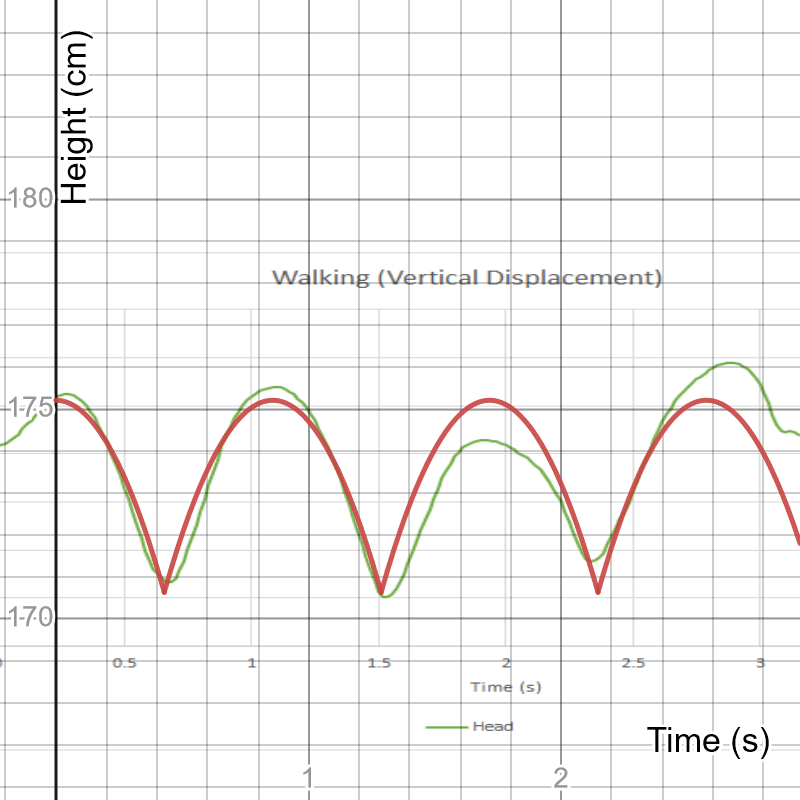
\includegraphics[width=10cm]{final_graph.png}
    \caption{ Graph of $h(x)$ overlaid over initial data collected.}
    \label{final_graph}
\end{figure}

It can be observed that even though the later steps do not quite reach the
maximum height due to the limited walking space available, the data is quite
nicely fit by the graph of $h(x)$, leading to the conclusion that the model is
accurate.

\subsubsection{Feet vertical oscillation}
To assemble the final model for the oscillation of the feet, it is a good start
to convert the quadratic $Q(x)$ into vertex form, as already shown.

\begin{align*}
    Q(x) &= -272.86x^2 + 981.44x -864.65 \\
         &\approx -272.86(x - 1.798)^2 + 17.876 \\
         &\therefore \text{Vertex at (1.798, 17.876)}
\end{align*}

It is also possible to find the x-coordinate of the inflection point of the
cubic $C(x)$ by finding the root of the second derivative.

\begin{align*}
        C(x) &= -493.51x^3+3120.52x^2-6577.99x+4633 \\
        \dv{C}{x} &= -1480.53x^2+6241.04x-6577.99 \\
        \dv[2]{C}{x} &= -2961.06x + 6241.04
\end{align*}

\begin{align*}
    -2961.06x + 6241.04 &= 0 \\
    -2961.06x  &= -6241.04 \\
    x &= \frac{-6241.04}{-2961.06} \\
    x &\approx 2.108
\end{align*}


\begin{figure}[H]
    \centering
    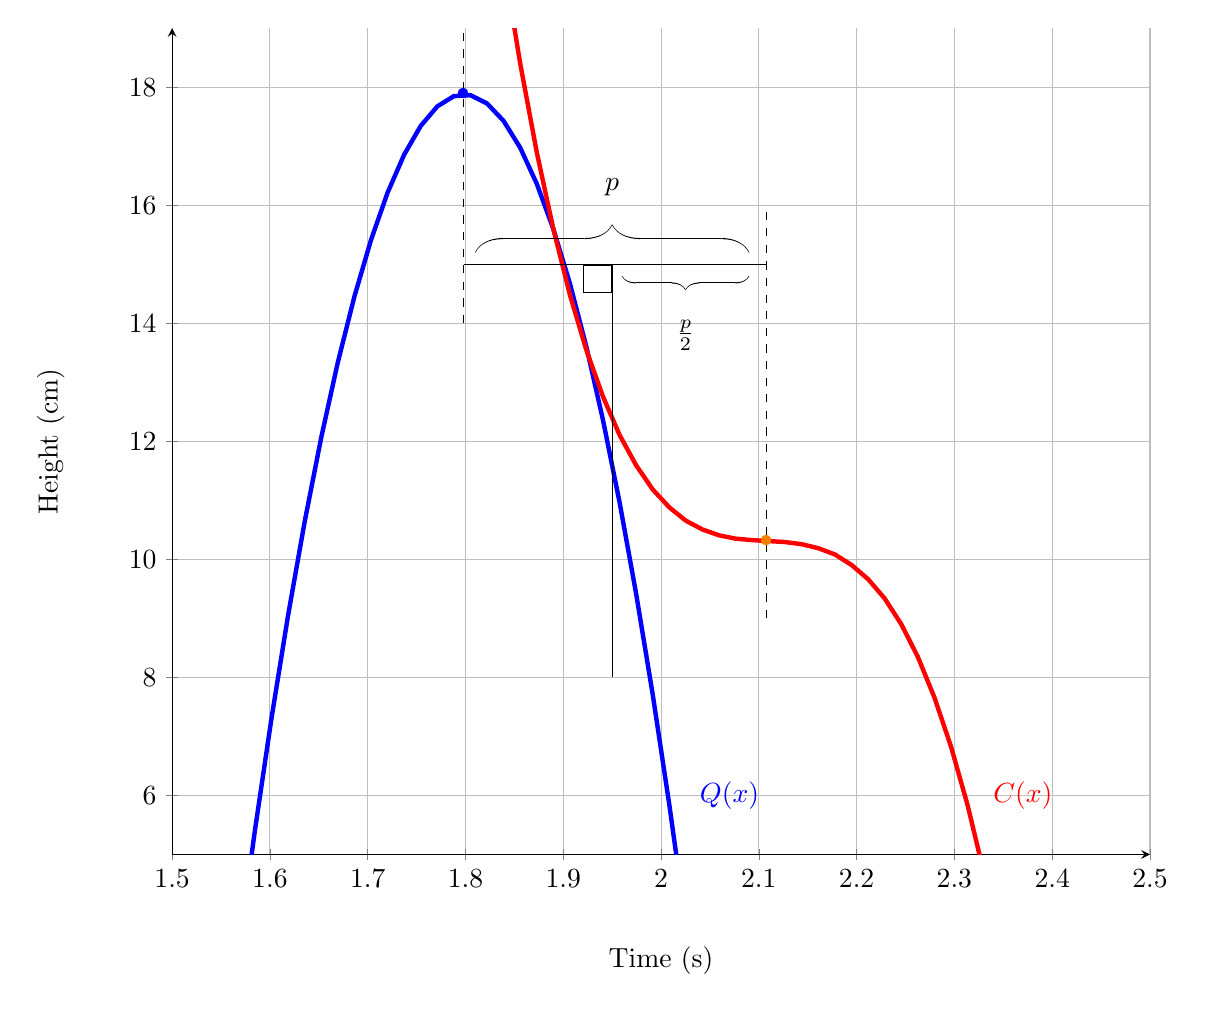
\begin{tikzpicture}
        \begin{axis}[
                axis y line=middle,
                axis x line=bottom,
                xmin=1.5,
                xmax=2.5,
                ymin=5,
                ymax=19,
                width=14cm,
                samples=60,
                no markers,
                grid,
                x label style={at={(axis description cs:0.5,-0.1)},anchor=north},
                y label style={at={(axis description cs:-0.1,.5)},rotate=90,anchor=south},
                xlabel={Time (s)},
                ylabel={Height (cm)},
            ]
            % quadratic
            \addplot [domain=1.5:2.5, ultra thick, blue] {-272.86*x^2+981.44*x-864.65};
            \node [blue] at (axis cs:2.07,6) {$Q(x)$};
            % cubic
            \addplot [domain=1.5:2.5, mark=none, ultra thick, red] {-493.51*x^3+3120.52*x^2-6577.99*x+4633};
            \node [red] at (axis cs:2.37,6) {$C(x)$};

            % vertex & inflection vline
            \draw [dashed] (axis cs:1.798,14) -- (axis cs:1.798,19);
            \draw [dashed] (axis cs: 2.108,9) -- (axis cs:2.108,16);
            
            % p line
            \draw [] (axis cs:1.798,15) -- (axis cs:2.108,15);
            
            % p
            \draw [decorate, decoration = {calligraphic brace, amplitude=10pt}] (axis cs:1.81,15.2) -- (axis cs:2.09,15.2);
            \node at (axis cs:1.95,16.3) {$p$};

            % p/2
            \draw [decorate, decoration = {calligraphic brace, mirror, amplitude=5pt}] (axis cs:1.96,14.8) -- (axis cs:2.09,14.8);
            \node at (axis cs:2.025,13.8) {$\frac{p}{2}$};

            % right angle
            % \draw[draw=black] (axis cs:1.95,14.5) rectangle ++(axis cs:1.5,1.5);

            \node (rect) at (axis cs:1.935,14.75) [draw,minimum width=3.5mm,minimum height=3.5mm] {};

            \node [blue] at (axis cs:1.798,17.876) {\textbullet};
            \node [orange] at (axis cs:2.108,10.311) {\textbullet};

            \draw [] (axis cs: 1.95,15) -- (axis cs:1.95,8);
        \end{axis}
    \end{tikzpicture}
    \caption{ Graphs of $Q$ and $C$. $d$ is the horizontal distance between the
        vertex of $Q$ and the inflection point of $C$. A perpendicular line
        bisects the created horizontal line at $d/2$ from either side. }
    \label{feetmodel}
\end{figure}

In order to express one peak as a single curve, first it can be expressed as a
piece wise $w(x)$ between the cubic and the quadratic, where the functions change
over at a horizontal distance $\frac{d}{2}$ away from the quadratic vertex's
x-coordinate $h$.

\[ w(x)= \begin{cases} -272.86(x-1.798)^2+17.876 & x \leq h + \frac{d}{2}\\
    -493.51x^3+3120.52x^2-6577.99x+4633 & x > h + \frac{d}{2} \\
\end{cases}
\]

However, this produces an undesired effect: the function is now discontinuous at
the meeting point $h+\frac{d}{2}$, which is not convenient if one wishes to use
this model to smooth some sort of movement as there would be a noticeable "bump"
where the functions change over. \\

In order to find a better place to put the meeting point, we can just equate the
cubic and quadratic, then solve for the roots of the resulting cubic. \\

\begin{align*}
    C(x) &= Q(x) \\
    -493.51x^3+3120.52x^2-6577.99x+4633 &= -272.86x^2 + 981.44x -864.65 \\
    -493.51 x^3 + 3393.38 x^2 - 7559.43 x + 5497.65 &= 0 \\
    \text{Solve using cubic formula, not shown for brevity} \\
    x \approx 1.89006 \qquad x \approx 1.926 \qquad x \approx 3.060\\
\end{align*}

We can pick any one of these values for the x-coordinate of the transition and
get a continuous graph, however the solution for $x \approx 3.060$ is beyond the
region of interest where we wish to join the functions together, so it can be
disregarded. From the solutions around 2, $x \approx 1.926$ has been chosen as
it appears to create a more smooth final function. Using this as a meeting
point, the piece wise function $w$ becomes:

\[ w(x)= \begin{cases} 
    -272.86(x-1.798)^2+17.876 & x \leq 1.926 \\
    -493.51x^3+3120.52x^2-6577.99x+4633 & x > 1.926
\end{cases}
\]


\begin{figure}[H]
    \centering
    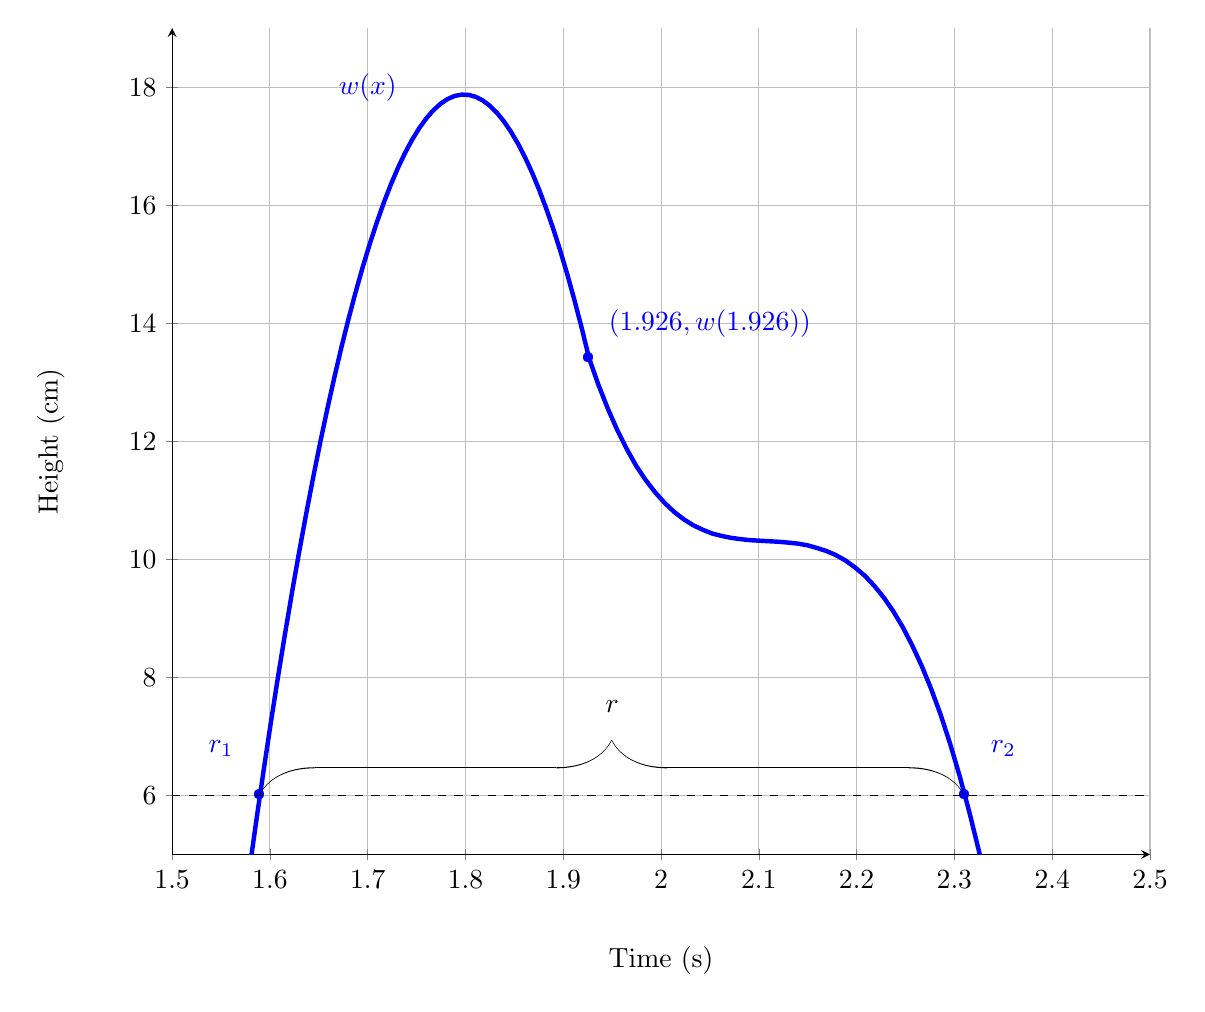
\begin{tikzpicture}
        \begin{axis}[
                axis y line=middle,
                axis x line=bottom,
                xmin=1.5,
                xmax=2.5,
                ymin=5,
                ymax=19,
                width=14cm,
                samples=60,
                no markers,
                grid,
                x label style={at={(axis description cs:0.5,-0.1)},anchor=north},
                y label style={at={(axis description cs:-0.1,.5)},rotate=90,anchor=south},
                xlabel={Time (s)},
                ylabel={Height (cm)},
            ]
            % quadratic
            \addplot [domain=1.5:1.926, ultra thick, blue] {-272.86*x^2+981.44*x-864.65};
            \addplot [domain=1.926:2.5, mark=none, ultra thick, blue] {-493.51*x^3+3120.52*x^2-6577.99*x+4633};
            \node [blue] at (axis cs:1.926,13.405) {\textbullet};
            \node [blue] at (axis cs:2.05,14) {$(1.926, w(1.926))$};
            \node [blue] at (axis cs:1.7,18) {$w(x)$};

            \node [blue] at (axis cs:1.55,6.8) {$r_1$};
            \node [blue] at (axis cs:1.589,6) {\textbullet};
            \node [blue] at (axis cs:2.35,6.8) {$r_2$};
            \node [blue] at (axis cs:2.31,6) {\textbullet};

            \draw [decorate, decoration = {calligraphic brace, amplitude=20pt}] (axis cs:1.589,6) -- (axis cs:2.31,6);
            \node at (axis cs:1.95,7.5) {$r$};

            \draw [dashed] (axis cs: 1.5,6) -- (axis cs:2.5,6);
        \end{axis}
    \end{tikzpicture}
    \caption{ Final graph of continuous $w(x)$, $r$ is the distance between the
    intersection points $r_1$ and $r_2$ of $w(x)$ with $y=6$ }
    \label{w(x)}
\end{figure}

As suggested by, Figure \ref{feet_y} the true "floor" of the graph of the
vertical oscillation in feet is actually above the x-axis. This is due to the
measurement being taken from the walker's ankle and not the very base of his
foot. Evidently, that point appears to about 6 cm above the true ground. We can
find the "roots" $r_1$ and $r_2$ by equating $w(x) = 6$. It would also be useful
to simply subtract 6 from the parts of $w$ in order to bring the floor to the
true $y=0$. Solving the equality yields the solutions $x \approx 1.589$ and
$x\approx 2.310$, giving us the values for $r_1$ and $r_2$. This, then, allows
us to calculate the value of $r$: $r = 2.310 - 1.589 \approx 0.721$. \\

The significance of $r$ is actually quite big. It was previously observed that
the "peaks" modeled by $w(x)$ alternate for each foot, meaning only one foot can
be undergoing a peak, while the other must be going through a plateau. This
means that the horizontal length of the peak we just found as $r$ must
correspond to a plateau on the graph of the other foot, therefore illustrating
that plateaus are of the same length as peaks. \\

Using this insight, it is now possible to model the final piece wise function
$h_{R}(x)$ for the vertical oscillation of the right foot. The function must be a
crest, followed by a trough, where both the crest and trough are $r$ units long
in the x-axis. The graph of $w$ should be translated horizontally so that $r_1$
is at the origin. This means that there would be a leftward horizontal
translation by $r_1$ units. Every pair of crests \& troughs, the graph of $w$
should also be translated to the right by $2r$ units.\\

\[ h_{R}(x)= \begin{cases} 
    w(x+r_1) & 0 \leq x < r \\
    0 & r \leq x < 2r \\[2mm]
    w(x + r_1 - 2r) & 2r \leq x < 3r \\
    0 & 3r \leq x < 4r \\[2mm]
    & \phantom{t=\,} \vdots
\end{cases}
\]

The function for the left foot $h_{L}(x)$ would simply be the above, but with
the order of the crests and plateaus swapped. This would effectively put the two
graphs completely out of phase, which is the desired effect.

\[ h_{L}(x)= \begin{cases} 
    0 & 0 \leq x < r \\
    w(x+r_1-r) & r \leq x < 2r \\[2mm]
    0 & 2r \leq x < 3r \\
    w(x+r_1-3r) & 3r \leq x < 4r \\[2mm]
    & \phantom{t=\,} \vdots
\end{cases}
\]

\begin{figure}[H]
    \centering
    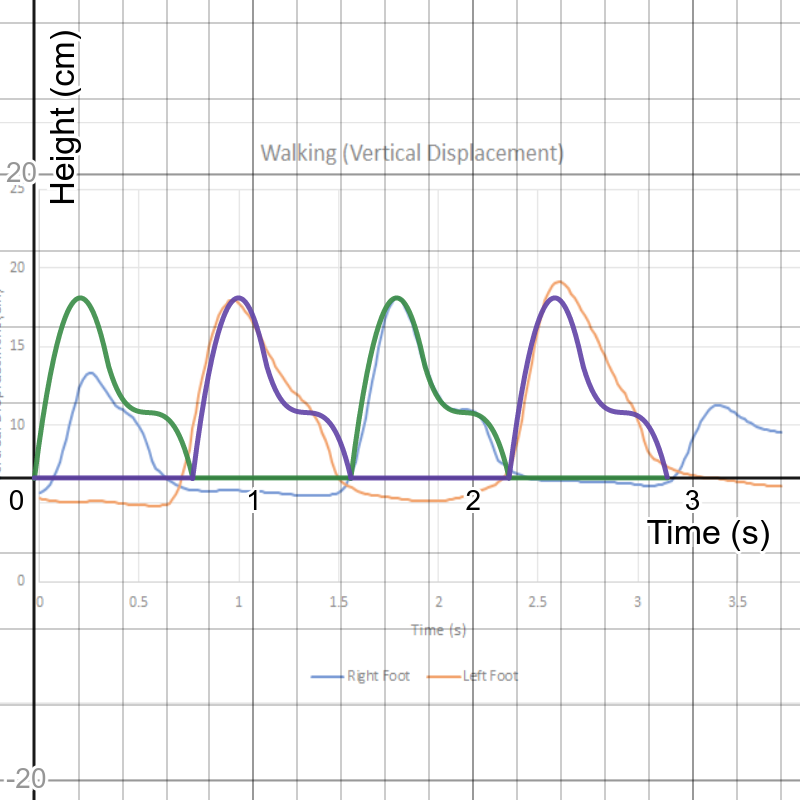
\includegraphics[width=10cm]{final_graph_feet.png}
    \caption{ Graph of $h_{R}(x)$ (green) and $h_{L}(x)$ (purple) overlaid over
    initial data collected.}
    \label{final_graph_feet}
\end{figure}

It is evident that the functions fit the three middle peeks well, with their
maximums \& points of transition lining up almost perfectly, which is indicative
of a strong model. Even though the first step did not reach the maximum height,
its features still line up horizontally with the fitted function which may
indicate that the misalignment is due to an external factor like the first step
not being as big as the rest.

\section{Evaluation \& conclusion}
From the models obtained for the vertical oscillation of both the head and feet
of a walking human, it is evident that polynomials are an effective way to model
the obtained data. However, it is important to note that the method through
which the polynomial is fitted to the graph plays a highly important role in the
accuracy of the final result. Each of the explored fitting methods has its own
strengths and limitations, so it is important to choose wisely for the dataset
at hand. \\

The models derived, themselves, may not necessarily have a high ecological
validity in that they describe the motion of one person's particular walking
style, which in and of itself is not particularly ensured to remain constant.
Although the model demonstrates malleability through its parameters, it would
potentially be worthwhile, as an extension, to add complexity based on more
granular real life physical properties of the person. \\

Furthermore, while the models fit to the dataset well in some regions, it would
potentially be meritous, as an extension to the work done here, to attempt to
model the dataset using a wave function like $y=\sin x$. While this would reduce
the accuracy of the fit in some places, it would produce a simpler definition of
the model which may be of benefit to some users seeking this simplicity over
overall accuracy. \\

In general, the resulting functions obtained throughout this investigation are
sufficient at modelling the vertical oscillation of the human body while
walking, and are therefore a good solution to the problem of this investigation.

\section{References}
Weisstein, E., 2022. Least Squares Fitting--Polynomial -- from Wolfram
MathWorld. [online] MathWorld. Available at:
https://mathworld.wolfram.com/LeastSquaresFittingPolynomial.html [Accessed
August 2022].

Weisstein, E., 2022. Least Squares Fitting -- from Wolfram MathWorld. [online]
MathWorld. Available at:
<https://mathworld.wolfram.com/LeastSquaresFitting.html> [Accessed August 2022].
\end{document}